%!TEX root = ../thesis.tex
\documentclass[..thesis.tex]{subfiles}

\begin{document}
Sampling profilers are a type of profiles which gather call traces from the observed program at varying intervals. A sample in the form of a call trace is a representation of a single thread's state at a particular moment in time. A simple call trace of a thread is presented in Listing ~\ref{lst:stack_trace}. 

\begin{lstlisting}[style=def,label={lst:stack_trace}, caption={Call trace of a thread}]
"main" #1 prio=5 os_prio=0 tid=0x00007feccc224000 nid=0x1f2c 
runnable [0x00007fecd5660000]
   java.lang.Thread.State: RUNNABLE
	    at ee.ut.SimpleBenchmark.methodA(SimpleBenchmark.java:28)
    	at ee.ut.SimpleBenchmark.doWork(SimpleBenchmark.java:22)
	    at ee.ut.SimpleBenchmark.main(SimpleBenchmark.java:11)
\end{lstlisting}

Gathered samples can then be aggregated and grouped based on their occurrence.
Distribution of the gathered samples highlights the hotspots in the program under observation. Higher frequency of a call trace suggests that more program's execution time was spent in that particular state. 

Figure \ref{fig:samplingProf} helps to visualize the performance implications of the frequency of the gathered samples. The visualization was created by a tool called Flamegraphs which provides means to generate a comprehensive and intuitive visualization of the gathered call trace samples \cite{gregg_flame}. Visualization tools are necessary to produce meaningful representations of the collected data as unprocessed call trace samples \textit{per se} are not informative without the context of other samples' frequency.

\begin{figure}[H]
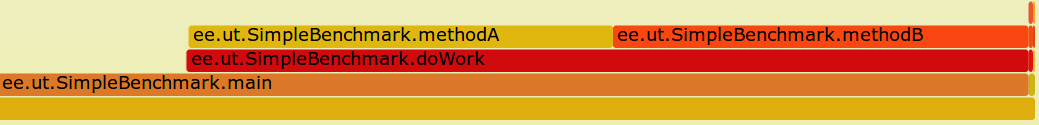
\includegraphics[scale=0.4]{equalsample.png}
\caption{Visualization of sampling profiling output}
\label{fig:samplingProf}
\end{figure}

The samples of the visualization in Figure \ref{fig:samplingProf} were gathered from a simple program that executed two identical methods, \texttt{methodA} and \texttt{methodB}, alternately. During its execution $481$ usable samples were collected. $198$ of those samples contained \texttt{methodA} in its top call frame and $194$ contained \texttt{methodB} in its top frame.

Although sampling profiling does not provide precise metrics for each method's execution time, it can provide a general overview to visualize the time spent in the profileable application's context. Such information is often sufficient to make actionable optimizations in the observed application.

\subsection{Importance of samples' quantity}

For sampling profilers, the result is a statistical approximation of the program's performance. Thus, having more samples will provide a more accurate approximation. 

Figure \ref{fig:lowSampleCount} illustrates the problem which is caused by the low sampling interval. Suppose that the Figure \ref{fig:lowSampleCount} resembles a program's execution in which the horizontal axis represents the current program's call trace state in that particular moment in time. It can be observed that the amount of time spent in method Y is significantly larger than the amount of time that was spent in methods X and Z. Suppose that the sampling profiler obtains a sample at each dotted vertical line. Such profiling results would represent each method X, Y and Z with a single sample. This implies that all the methods spent roughly the same amount of time during the execution of the program. The result is inaccurate as the visualization clearly shows that method Y spent roughly 4 times more time than it was spent for executing methods X and Z.

\begin{figure}[H]
\centering
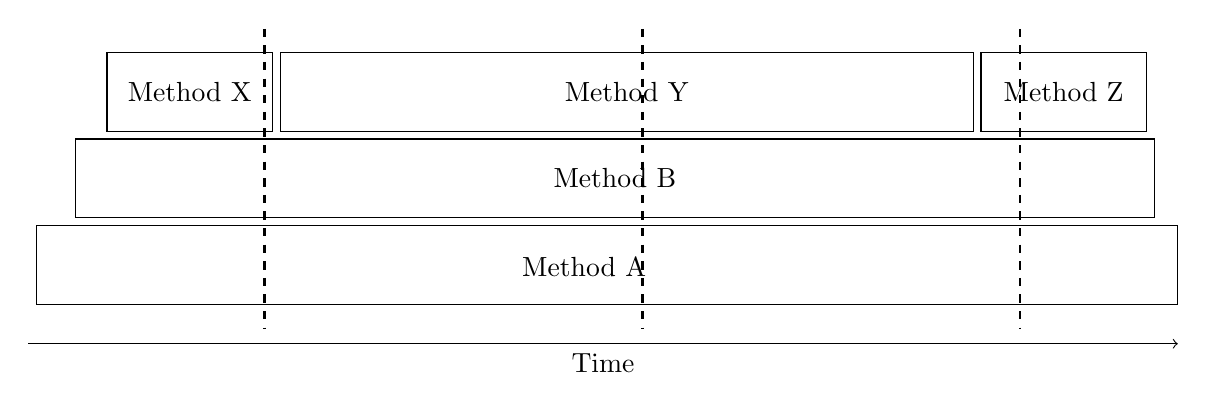
\begin{tikzpicture}
% Call stack rectangles
\draw (0,0) rectangle (14.5,1) node[pos=.48] {Method A};
\draw (0.5,1.1) rectangle (14.2,2.1) node[pos=.5] {Method B};

\draw (0.9,2.2) rectangle (3,3.2) node[pos=.5] {Method X};
\draw (3.1,2.2) rectangle (11.9,3.2) node[pos=.5] {Method Y};
\draw (12.0,2.2) rectangle (14.1,3.2) node[pos=.5] {Method Z};

% x-axis time arrow below
\draw[->] (-0.1,-0.5) -- (14.5, -0.5) node[below, pos=.5] {Time};

% samples
\draw[dashed, thick] (2.9,3.5) -- (2.9,-0.3);
\draw[dashed, thick] (7.7,3.5) -- (7.7,-0.3);
\draw[dashed, thick] (12.5,3.5) -- (12.5,-0.3);

\end{tikzpicture}
\caption{Scenario with low sampling interval}
\label{fig:lowSampleCount}
\end{figure}

Increasing the sampling interval would improve the situation as demonstrated on Figure \ref{fig:highSampleCount} on page \pageref{fig:highSampleCount}. Upon profiling with a four times higher sampling interval, it becomes apparent that method Y call trace samples have been proportionally represented in the total call trace samples. The call trace samples containing the method Y in its top frame are colored red on the Figure \ref{fig:highSampleCount}.

\begin{figure}[H]
\centering
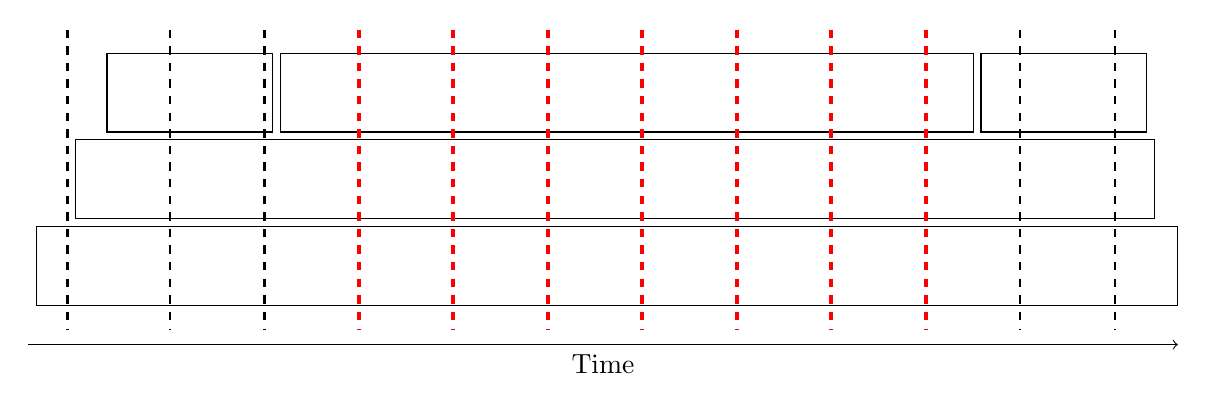
\begin{tikzpicture}
% Call stack rectangles
\draw (0,0) rectangle (14.5,1) node[pos=.48] {};
\draw (0.5,1.1) rectangle (14.2,2.1) node[pos=.5] {};

\draw (0.9,2.2) rectangle (3,3.2) node[pos=.5] {};
\draw (3.1,2.2) rectangle (11.9,3.2) node[pos=.5] {};
\draw (12.0,2.2) rectangle (14.1,3.2) node[pos=.5] {};

% x-axis time arrow below
\draw[->] (-0.1,-0.5) -- (14.5, -0.5) node[below, pos=.5] {Time};

% samples
\draw[dashed, thick] (0.4,3.5) -- (0.4,-0.3);
\draw[dashed, thick] (1.7,3.5) -- (1.7,-0.3);
\draw[dashed, thick] (2.9,3.5) -- (2.9,-0.3);

\draw[red, dashed, line width=0.5mm] (4.1,3.5) -- (4.1,-0.3);
\draw[red, dashed, line width=0.5mm] (5.3,3.5) -- (5.3,-0.3);
\draw[red, dashed, line width=0.5mm] (6.5,3.5) -- (6.5,-0.3);
\draw[red, dashed, line width=0.5mm] (7.7,3.5) -- (7.7,-0.3);
\draw[red, dashed, line width=0.5mm] (8.9,3.5) -- (8.9,-0.3);
\draw[red, dashed, line width=0.5mm] (10.1,3.5) -- (10.1,-0.3);
\draw[red, dashed, line width=0.5mm] (11.3,3.5) -- (11.3,-0.3);

\draw[dashed, thick] (12.5,3.5) -- (12.5,-0.3);
\draw[dashed, thick] (13.7,3.5) -- (13.7,-0.3);

\end{tikzpicture}
\caption{Scenario with sufficient sampling interval}
\label{fig:highSampleCount}
\end{figure}

\subsection{Sampling profiling challenges}
There are multiple problems that the implementations of sampling profilers could experience. These problems could potentially affect the reliability of the samples provided by the sampling profiler.

% \supervisor{I would write out what you mean under results here, although not as important is in introduction as }
\subsubsection{Periodicity bias}
This problem occurs when the sampling interval catches on to some program's routine which executions match the sampling interval. Figure \ref{fig:periodicityBias} illustrates the issue behing the bias. Suppose that the program to be observed runs \texttt{Method X} and \texttt{Method Y} alternatingly for some constant time period. If the dotted lines are the marks for the call trace samples taken during profiling, the results would be skewed as not a single sample represents \texttt{Method Y} in the results. 

\begin{figure}[H]
\centering
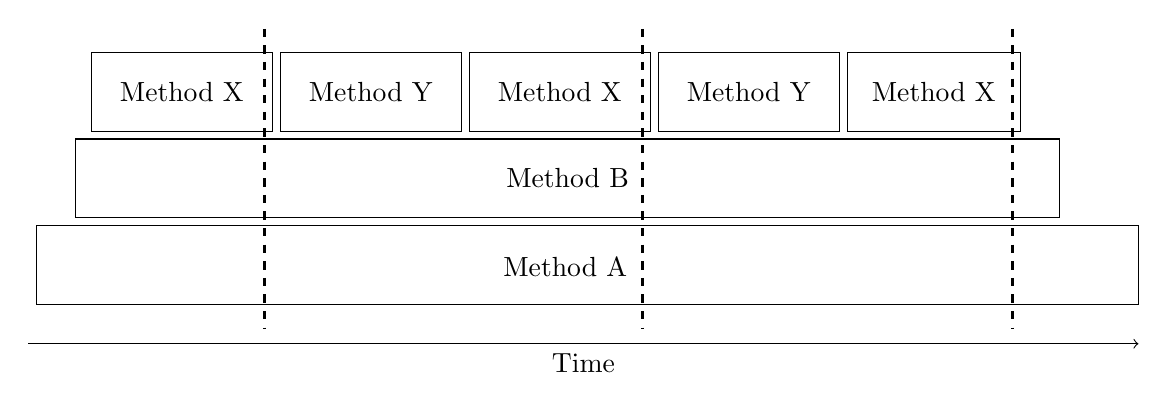
\begin{tikzpicture}
% Call stack rectangles
\draw (0,0) rectangle (14,1) node[pos=.48] {Method A};
\draw (0.5,1.1) rectangle (13,2.1) node[pos=.5] {Method B};
\draw (0.7,2.2) rectangle (3,3.2) node[pos=.5] {Method X};
\draw (3.1,2.2) rectangle (5.4,3.2) node[pos=.5] {Method Y};
\draw (5.5,2.2) rectangle (7.8,3.2) node[pos=.5] {Method X};
\draw (7.9,2.2) rectangle (10.2,3.2) node[pos=.5] {Method Y};
\draw (10.3,2.2) rectangle (12.5,3.2) node[pos=.5] {Method X};

% x-axis time arrow below
\draw[->] (-0.1,-0.5) -- (14, -0.5) node[below, pos=.5] {Time};

% samples
\draw[dashed, thick] (2.9,3.5) -- (2.9,-0.3);
\draw[dashed, thick] (7.7,3.5) -- (7.7,-0.3);
\draw[dashed, thick] (12.4,3.5) -- (12.4,-0.3);

\end{tikzpicture}
\caption{Illustration of periodicity bias}
\label{fig:periodicityBias}
\end{figure}

Possible way to tackle this problem would be to randomize the sampling interval by having a random number of time units offseting the sampling interval. Increasing sample gathering frequency will also help to alleviate this problem.

\subsubsection{Safepoint bias}
Sampling profiling assumes that the obtained samples are acquired uniformly and randomly as bias in the samples could potentially yield inaccurate results. In light of this, when gathering samples from a program running on the Java Virtual Machine, one must take \textit{safepoints} into consideration.

Safepoints in the Java Virtual Machine are defined as points during the program's execution during which all of the threads are in a consistent and well known state. Safepoints are necessary for various Java Virtual Machine's operations such as the garbage collection, method deoptimization and class redefinition.\cite{hotspot_glossary} It has been shown that most of the existing Java profilers require the Java Virtual Machine to be stopped on a safepoint in order to obtain the call trace sample from the profileable thread \cite{wakart_psychosomatic_2016}. However, this mechanism also casts a shadow on the profling results as this implies that the samples are not acquired randomly but rather require the Java Virtual Machine to be in a specific state \cite{mytkowicz_evaluating_2010}. 

The execution of the code sample in Listing ~\ref{lst:safepoint} illustrates this issue well. The nested loop in this example is to avoid Java compiler specific optimizations.

\begin{lstlisting}[language=java,style=def,label={lst:safepoint}, caption={Counted loops do not contain safepoints}]
int k = 0;
for (int i = 0; i < Integer.MAX_VALUE; i++) {
	for (int j = 0; j < 2; j++) {
    	k++;
    	if ((k % 2) == 1) k++;
	}
}
\end{lstlisting}
As various Java Virtual Machine routines are nondeterministic, it is impossible to predict when does the Java Virtual Machine signal its threads to be stopped on a safepoint. However, if such request should occur in the middle of the counted loop's execution in Listing \ref{lst:safepoint}, the thread executing the loop's instructions will not stop until the loop has finished. Thus, if an ordinary sampling profiler signals the thread for a call trace sample, it is delayed until the thread executing the loop's instructions finishes its task \cite{wakart_psychosomatic_2015}. 

To measure the actual time that is spent waiting for the Java Virtual Machine to stop all its threads on a safepoint, \texttt{-XX:+PrintGCApplicationStoppedTime} flag can be used. Appending this flag to the Java Virtual Machine arguments, it enables outputing the time it takes for the Java Virtual Machine to stop all threads in order to execute a subroutine and the time that this operation took in total. Due to nondeterminicity, the sample code in Listing \ref{lst:safepoint} was executed $100$ times. The worst case among $100$ program executions recorded a Java Virtual Machine operation that took $7.517$ seconds and $99.999\%$ of that time was spent on reaching a safepoint. It is worth mentioning that this operation took $65\%$ of the whole program's execution time.

% \supervisor{of this scale -- I doubt that the bias is rare, just that it usually is small}
Although the provided example is rather artificial and such occurrences in real life programs are rare on such large scale, it clearly points out the bias that the safepoints potentially introduce. Such bias during obtaining the call trace clearly contradicts the randomness prerequisite for sampling profiling. Despite the presence of safepoint bias, such profiler can still produce actionable profiling results but lessen the accuracy when high detail granularity of the results is important.

\subsubsection{Observer effect}

Attaching a profiler to an application does alter the way how the application would normally execute. The \textit{observer effect} describes how a presence of a profiler can change the profiling outcome.
 
Firstly, a profiler does introduce some performance overhead due to its nature. Profilers do need to execute additional instructions for gathering information from the application under observation. To have meaningful profiling results, this overhead must not affect the application's performance by a large margin.

%  \supervisor{This is undefined definition at this point. Maybe try to give a simple defitiniot beforehand? something ``in contrast to sampling profiler'' Or try to move some of the definition in next paragraph earlier?} 

\TODO{Check phrasing of the following paragraph with supervisors}
The presence of a profiler could also change the way how the Java Virtual Machine does its optimizations. Java Virtual Machine makes use of just-in-time (JIT) compilation techniques during at run time. JVM identifies methods which meet some criterias (e.g. called frequently) and compiles these methods into native machine code, resulting in an highly optimized code which improves the performance of such methods \cite{understanding_jit}. Various information extracting functions might change the way how the bytecode on the Java Virtual Machine is executed \cite{mytkowicz_evaluating_2010}. The presence of a profiler could alter which methods are eligible for JIT compilation. Thus, resulting in a different performance profile when compared to an application's execution in which the profiler is not attached.

%This factor affects sampling profilers as well but it is especially relevant for tracing profilers 

\subsection{Sampling profiling compared to alternatives}

An alternative approach for gathering performance information is using tracing profilers. Tracing profilers rely on instrumenting the bytecode of the profileable application. In the context of tracing profilers, instrumentation is the act of adding additional instructions to the application being observed in order to gather relevant profiling information. Tracing profilers instrument the observed application by wrapping method calls with instructions to measure method execution time. Result is a collection of call stacks with included precise method timings \cite{whitham_jack}. Simplified idea of tracing profiler instrumentation is shown on Figures ~\ref{lst:uninstrumented} and \ref{lst:instrumented}. Figure \ref{lst:uninstrumented} shows the source code of a simple method and Figure \ref{lst:instrumented} shows how a tracing profiler could instrument the code shown on Figure \ref{lst:uninstrumented} in order to obtain information about method execution time.

\begin{minipage}[b]{.45\textwidth}
\begin{lstlisting}[language=java,style=def,label={lst:uninstrumented}, caption={Original source}]
public void work() {
  doWork();
}
\end{lstlisting}
\end{minipage}\hspace{12mm}
\begin{minipage}[b]{.45\textwidth}
\begin{lstlisting}[language=java,style=def,label={lst:instrumented}, caption={Instrumented source}]
public void work() {
  long start = System.nanoTime();
  doWork();
  long end = System.nanoTime() - start;
  // Profiler then persists the `end` value
}
\end{lstlisting}
\end{minipage}
%[language=java,style=def,label={lst:safepoint}, caption={Counted loops do not contain safepoints}]



Using tracing profilers usually requires the user or the profiler to know the application elements that are worth profiling as instrumenting all the methods in the application under observation is too expensive performance wise. 

Downside of tracing profiling is its performance and its susceptibility to observer effect. Tracing profilers rely on bytecode instrumentation which directly affects the way how the Java Virtual Machine performs its optimizations. Some optimizations might not be possible due to the added bytecode instructions added by the tracing profiler. Additionally, depending on the level of information detail and the amount of instrumentation performed, requiring higher information granularity could potentially introduce impactful overhead to the application's performance which could result in inaccurate profiling results. 

When comparing sampling profiling to tracing profiling, it excels with its performance. Sampling profilers can potentially obtain thousands of samples each second with negligible performance overhead.

\subsection{Sampling profiling possible implementations for the JVM}

\subsubsection{\texttt{jstack}}
\texttt{jstack} is an utility included in the Oracle's JDK and OpenJDK by default. This utility can be used to print out stack traces of all threads of a Java process \cite{jstack}. The simplest implementation to show the concept of a sampling profiler would be to periodically call the \texttt{jstack} utility to obtain the snapshot of all threads. These snapshots can be persisted and processed to produce a visualization of the application's performance. This approach has a relatively high overhead when compared to other sampling profiling methods and is not a viable method for profiling real world applications but rather illustrates the concept of sampling profiling.

\subsubsection{\texttt{GetAllStackTraces} profilers}
\texttt{GetAllStackTraces} is a method in the official JVM Tooling Interface (JVMTI) which is a programming interface utilized by development and monitoring tools. This method enables the profiler to extract the stack traces of all the threads currently executing on the JVM \cite{jvmtm}. Downside for this method is the fact that profilers utilizing this method are safepoint biased. For this reason, the performance is negatively affected due to frequent pauses for reaching safepoints.

Due to safepoint induced performance problems, this method aquired significantly less samples when compared to profilers based on \texttt{Async\-Get\-Call\-Trace}. Additionally, profiling results might be biased due to the fact that the stack traces can only be obtained when the JVM has reached a safepoint.

\texttt{GetAllStackTraces} is used in most commercial profilers such as JVisualVM, YourKit and JProfiler \cite{wakart_psychosomatic_2016, visualvm}.  


\subsubsection{\texttt{AsyncGetCallTrace} profilers}
%\supervisor{Maybe a bit how it enables obtaining such a call trace, and that it is meant to be called from signal handlers (and hence he Asynch part)?}

These kind of profilers make use of an undocumented JVM method \texttt{Async\-Get\-Call\-Trace} which enables obtaining call traces from a thread without the safepoint bias \cite{agct_source}. The asynchronous nature of this method enables the profiler to safely call this method in a signal handler which is the key architectural element for these kind of profilers \cite{signal-safety7}.

Due to safepoint bias free sample obtaining method, profiling samples tend to be more accurate since the JVM does not have to stop on a safepoint in order to obtain the call trace of the running thread. This method is a part of the JVMTI API.

Notable examples of such profilers which utilize \texttt{Async\-Get\-Call\-Trace} method  are Honest Profiler and Java Mission Control. 

\subsubsection{Native profilers}
%\supervisor{Connect the two sentences more strongy, like ``The main downside being'' or somethnig.}
Native profilers are tools utilizing the low level abstractions of the operating system to  profile the native binaries for the operating system. These profilers are superior to the previously described methods performance wise but do fall short on the usefulness of the gathered information. The main downside of native profilers is the inability obtain sufficient information about the Java level stack frames executed inside the Java Virtual Machine. Unlike other sampling techiniques introduced, native profilers are not much use to profile applications running on the Java Virtual Machine where most of the code has not been optimized yet.

%\TODO{Add example of native call trace to show that it is kind of useless} \supervisor{To be fair, one would have to give a sample such as one used with perf-map-agent}

%\supervisor{I would not bring in more here, let's leave it out of scope. Maybe add that ``unlike other sampling techiniques introduced, native profilers are not much use to debug a JVM where most of the code has not been yet optimized'' or something similar, to give a reason why we leave those out.} 
\end{document}
